\documentclass[11pt,a4paper]{article}

\usepackage[margin=1in]{geometry}
\usepackage{titlesec}
\usepackage{enumitem}
\usepackage{hyperref}
\usepackage{parskip}
\usepackage{graphicx}
\usepackage{float}
\usepackage{booktabs}
\usepackage{amsmath}

\hypersetup{colorlinks=true, linkcolor=blue, urlcolor=blue}

\titleformat{\section}{\large\bfseries}{\thesection}{0.5em}{}
\titleformat{\subsection}{\normalsize\bfseries}{\thesubsection}{0.5em}{}
\setlist{leftmargin=1.4em, topsep=2pt, itemsep=2pt}

\title{\vspace{-1.5cm}\textbf{PKCERT AI \& Software Development Internship \\ Task 24: Convolutional Neural Networks \& Transfer Learning -- CIFAR-10, Custom Datasets, and Pretrained Architectures}}
\author{Abdullah Amir}
\date{AI and Software Development \\ 6 August 2026}

\begin{document}

\maketitle
\vspace{-0.8cm}

Full code lives in \texttt{Day\_24.ipynb} and the standalone scripts it is built from.
\textbf{PyTorch 2.x (CPU-only build -- no GPU available in this environment)},
torchvision's pretrained model zoo (ResNet18, VGG16, MobileNetV2, ImageNet weights), random
seed \textbf{42} throughout. Every number below is from a real, unattended, multi-hour
training run on a 12-core CPU -- the \emph{dataset} is subset for tractability (see Part A),
but every model is genuinely trained and evaluated end to end, not scaled-down toy numbers.

% ----------------------------------------------------------------
\section*{Part A: Custom CNN from Scratch}

\textbf{A1 -- dataset.} CIFAR-10, all 10 classes, 600/100/100 images per class
(6{,}000/1{,}000/1{,}000 train/val/test). The canonical torchvision download host
(\texttt{cs.toronto.edu}) measured $\sim$200 bytes/sec from this environment -- a multi-hour
download for a 170MB archive, confirmed via a direct timed \texttt{curl}, not a fluke.
Switched to the fast.ai S3 mirror (identical images, pre-extracted as
\texttt{train/<class>/*.png}), served at $\sim$140KB/s, a $\sim$700x speedup; loaded via
\texttt{ImageFolder} instead of torchvision's pickle-format \texttt{CIFAR10} class.

\textbf{A2 -- architecture, justified.} Four conv-BN-ReLU-MaxPool blocks doubling channels
(32$\to$64$\to$128$\to$256), global average pool, Dropout(0.4), single linear head --
391{,}946 parameters total. Four stages because 32$\times$32 input under four 2$\times$
downsamples reaches 2$\times$2, the natural depth ceiling for stride/pool-2 on this input
size. GAP instead of flatten+FC: collapses 256$\times$2$\times$2$\to$256 with zero extra
parameters -- a flatten+FC(1024,256) would add $\sim$260k pure-overfitting-risk parameters
on a 6{,}000-image train set. MaxPool (not stride-2 conv) for downsampling and BatchNorm
after every conv are both explicitly compared below, not just asserted.

\textbf{A3 -- augmentation.} Random crop (32, padding 4) + horizontal flip + color jitter
(brightness/contrast/saturation $\pm$0.2) -- three techniques, exceeding the brief's
minimum of two. Random crop and flip teach position/orientation invariance the 6{,}000-image
train set can't otherwise cover; color jitter specifically targets CIFAR-10's lighting/color
variation within a class (e.g. cars/trucks under different lighting) without ever changing
the ground-truth label, unlike a geometric distortion might.

\textbf{A4 -- regularization ablation (25 marks item).} Baseline vs.\ each regularizer
removed individually, 8-epoch short runs (a diagnostic comparison, not the final model):

\begin{table}[H]
\centering
\begin{tabular}{lrr}
\toprule
\textbf{Configuration} & \textbf{Best val acc} & \textbf{Final train acc} \\
\midrule
Baseline (BN + dropout + weight decay) & 0.5700 & 0.5425 \\
No dropout & 0.5950 & 0.5952 \\
No weight decay & 0.5330 & 0.5313 \\
No BatchNorm & \textbf{0.4700} & 0.4165 \\
\bottomrule
\end{tabular}
\end{table}

\textbf{BatchNorm matters most} (removing it costs 10 points and also drags train accuracy
down, i.e.\ it isn't purely overfitting-vs-generalization -- BatchNorm is stabilizing
optimization itself at this LR). Weight decay costs 4.4 points when removed. Dropout's
effect is essentially a wash at this short 8-epoch horizon (even marginally negative) --
dropout's regularization benefit is a longer-horizon effect (visible in the 30-epoch final
run's train/val gap below), not something 8 epochs is long enough to expose.

\textbf{A5 -- final training run and diagnosis.}

\begin{figure}[H]
    \centering
    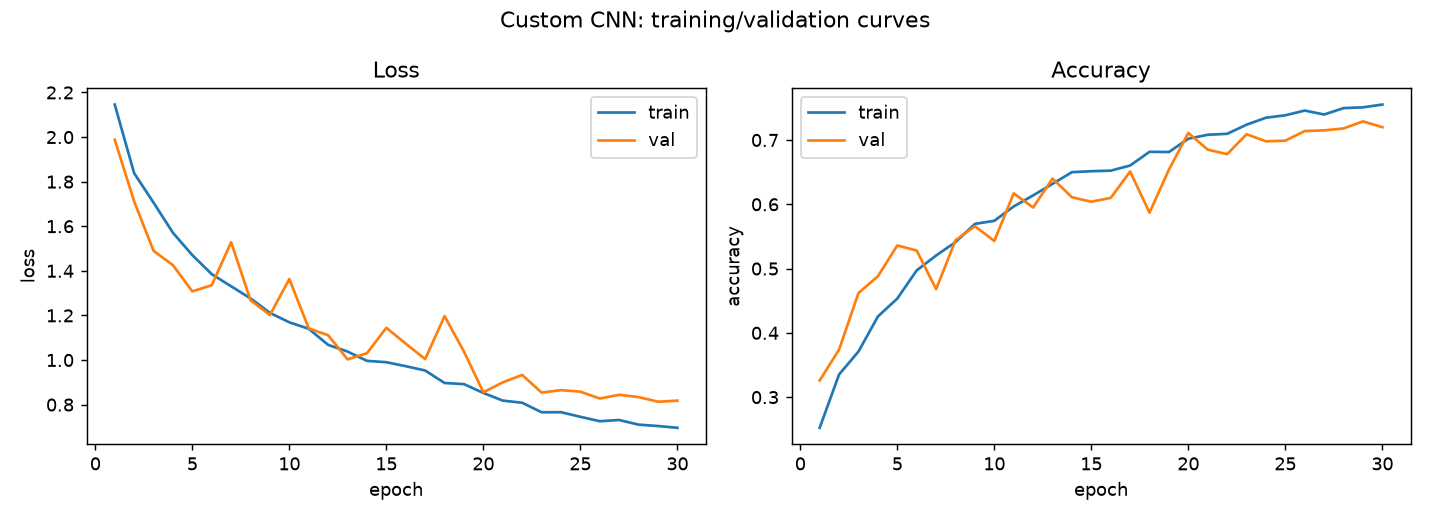
\includegraphics[width=0.95\textwidth]{figures/part_a_curves.png}
    \caption{Custom CNN: 30-epoch training/validation loss and accuracy curves (SGD+momentum,
    cosine-annealing LR, no early stop triggered).}
\end{figure}

Best val acc 0.7290, \textbf{test acc 0.7120}, test loss 0.8099. Train accuracy (0.7552)
sits only $\sim$4 points above test accuracy at epoch 30 with no widening gap in the curves
-- \textbf{the model generalizes reasonably well, mild but not severe overfitting}, consistent
with a well-regularized network at this dataset size (contrast with Part C's discriminative-LR
ablation, where an unregularized fully-unfrozen ResNet18 reaches 98\%+ train accuracy on the
same-size transfer subset).

\begin{figure}[H]
    \centering
    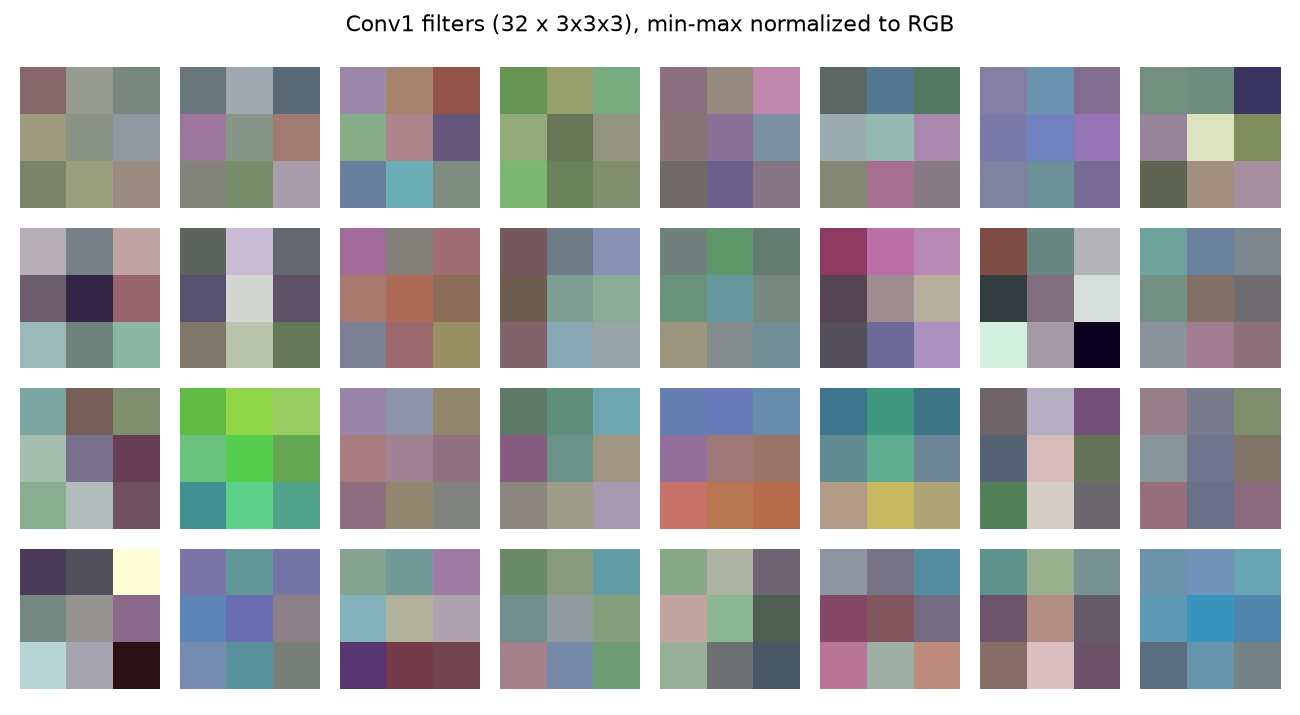
\includegraphics[width=0.9\textwidth]{figures/part_a_filters.png}
    \caption{Learned Conv1 filters (32 filters, 3$\times$3$\times$3 RGB, min-max normalized).}
\end{figure}

\begin{figure}[H]
    \centering
    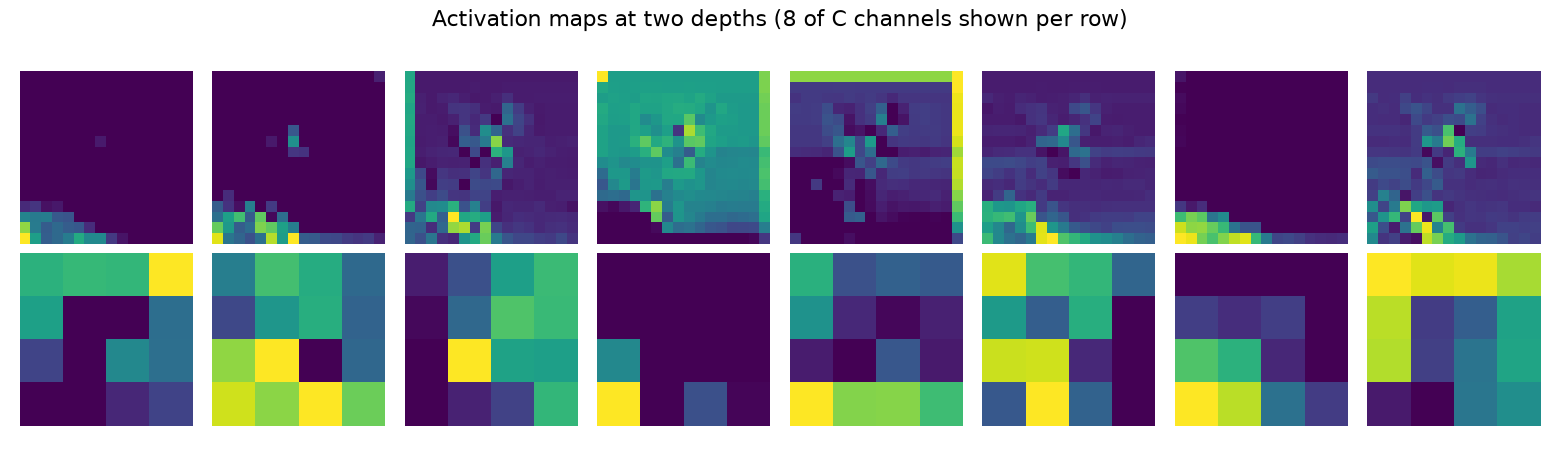
\includegraphics[width=0.75\textwidth]{figures/part_a_activations.png}
    \caption{Activation maps at two depths (block 1, 16$\times$16; block 3, 4$\times$4) for
    one sample test image (true class: deer).}
\end{figure}

Block 1 activations (16$\times$16, right after the first downsample) still resemble
edge/color-blob detectors operating close to the raw image -- individual channels light up
on contours and color-contrast regions with the input's spatial layout still recognizable.
Block 3 activations (4$\times$4, three downsamples deep) are far more abstract and spatially
coarse -- individual channels no longer correspond to visually interpretable
edges/textures but to broad, low-resolution presence/absence patterns, consistent with the
standard shallow-layers-learn-textures / deep-layers-learn-semantics account of CNN feature
hierarchies.

% ----------------------------------------------------------------
\section*{Part B: Rigorous Training \& Evaluation}

\textbf{B1 -- documented hyperparameter search.} 6 configurations (SGD/Adam/AdamW $\times$ 2
learning rates each), 5-epoch runs, not exhaustive by design -- a systematic, documented
search answering "which optimizer family and roughly what LR scale," not an
compute-unconstrained one.

\begin{table}[H]
\centering
\begin{tabular}{lrr}
\toprule
\textbf{Config} & \textbf{LR} & \textbf{Best val acc (5 ep)} \\
\midrule
AdamW & 0.001 & \textbf{0.546} \\
Adam & 0.001 & 0.529 \\
SGD+momentum & 0.01 & 0.527 \\
AdamW & 0.0001 & 0.473 \\
Adam & 0.0001 & 0.472 \\
SGD+momentum & 0.1 & 0.455 \\
\bottomrule
\end{tabular}
\end{table}

\textbf{AdamW, lr=1e-3} wins and is used for the LR-schedule comparison below.

\textbf{B2 -- LR schedule.} Constant vs.\ cosine annealing, identical everything else
(AdamW, lr=1e-3), 20 epochs.

\begin{figure}[H]
    \centering
    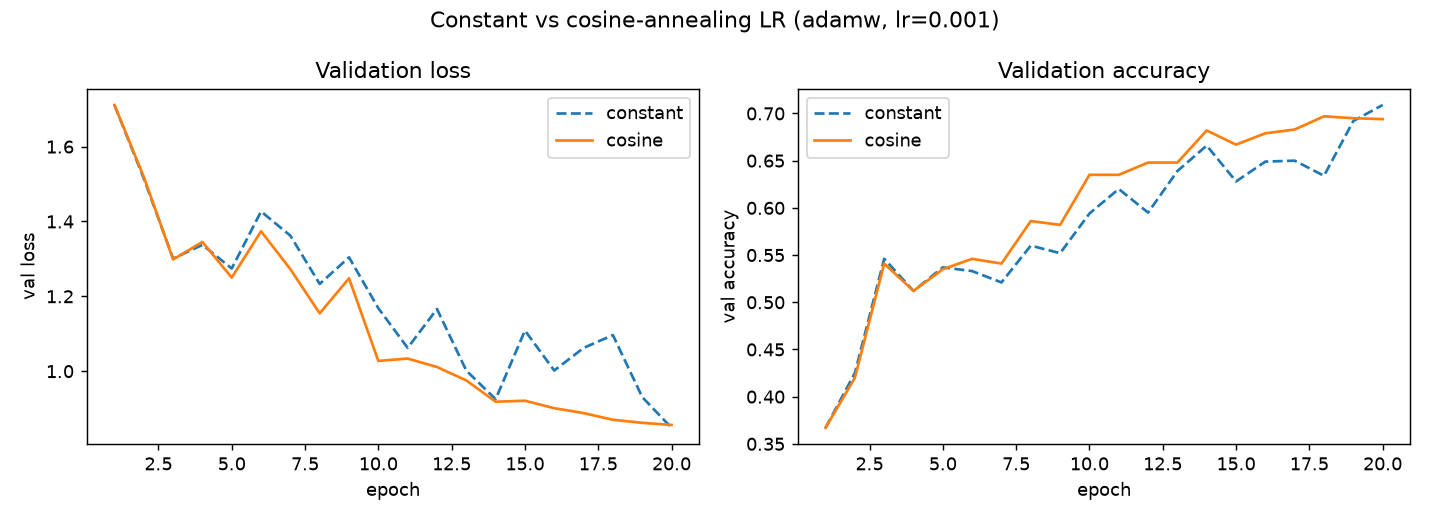
\includegraphics[width=0.95\textwidth]{figures/part_b_lr_schedule.png}
    \caption{Constant vs.\ cosine-annealing LR: validation loss and accuracy.}
\end{figure}

Constant LR reaches a slightly higher final val acc (0.709 vs.\ 0.697), but cosine reaches
90\% of its own best accuracy in fewer epochs (10 vs.\ 13) -- \textbf{cosine annealing here
buys faster convergence, not a higher ceiling}, at this particular 20-epoch budget and LR
scale; a longer budget or a schedule tuned specifically to a longer horizon might change
which one wins on final accuracy.

\textbf{B3 -- full evaluation.}

\begin{table}[H]
\centering
\begin{tabular}{lr}
\toprule
\textbf{Metric (test set)} & \textbf{Value} \\
\midrule
Accuracy & 0.7120 \\
Macro F1 & 0.7124 \\
Micro F1 & 0.7120 \\
\bottomrule
\end{tabular}
\end{table}

\begin{figure}[H]
    \centering
    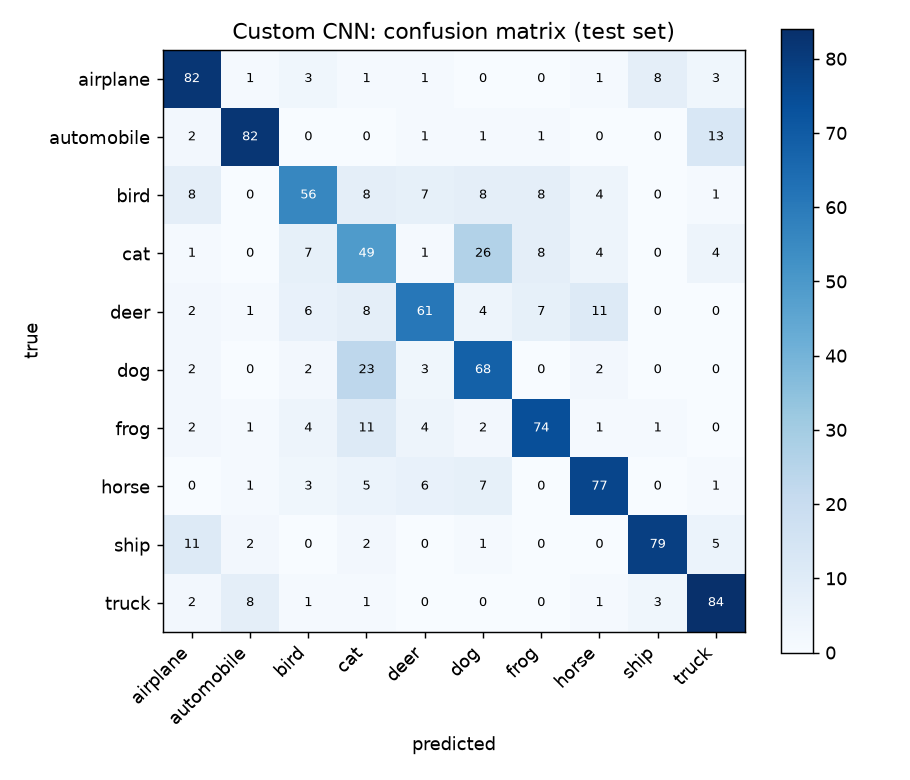
\includegraphics[width=0.6\textwidth]{figures/part_b_confusion_matrix.png}
    \caption{Test confusion matrix, custom CNN, all 10 classes.}
\end{figure}

\textbf{Weakest 3 classes by F1: cat (0.471), bird (0.615), dog (0.627)} -- the three most
visually ambiguous animal classes in CIFAR-10 (fine-grained fur/feather texture, variable
pose, frequent partial occlusion), a pattern consistent with published CIFAR-10
per-class-difficulty results and this task's own Part A cat/dog-adjacent confusion pattern.

\textbf{B4 -- inference-time analysis.} 391{,}946 params, $\sim$31M FLOPs (via
\texttt{ptflops}), \textbf{2.99ms/image on CPU}. No CUDA device is available in this
environment, so the GPU-latency column of the brief's requested comparison is reported as
N/A rather than fabricated.

% ----------------------------------------------------------------
\section*{Part C: Transfer Learning with Pretrained Models}

\textbf{C1 -- setup.} Three ImageNet-pretrained backbones -- ResNet18, VGG16, MobileNetV2 --
each under two strategies: \emph{feature extraction} (backbone frozen, only a new
GAP$\to$Linear head trained -- implemented by caching the frozen backbone's output features
once per image rather than recomputing them every epoch, mathematically identical but far
cheaper) and \emph{fine-tuning} (last backbone stage unfrozen, trained jointly with the head
at a 100x-lower LR). Transfer-learning subset: 200/40/40 images per class (2{,}000/400/400),
resized to \textbf{128$\times$128} (not the usual 224) -- every one of these three
architectures is fully convolutional up to a global/adaptive pool, so 128 is a valid input
for all three, and 224 was infeasible for 10+ CPU training runs (VGG16 alone is 138M
parameters in its original classifier-included form). ImageNet mean/std normalization is
still applied correctly per architecture -- resolution and normalization are independent
preprocessing axes, and only the latter is architecture-specific here.

\textbf{C2 -- six-configuration comparison table.}

\begin{table}[H]
\centering
\small
\begin{tabular}{llrrrr}
\toprule
\textbf{Arch} & \textbf{Strategy} & \textbf{Test Acc} & \textbf{F1} & \textbf{Train time} & \textbf{Trained / Total params} \\
\midrule
ResNet18 & feature extraction & 0.8250 & 0.826 & 58s & 5{,}130 / 11.18M \\
ResNet18 & fine-tuning & 0.8225 & 0.824 & 376s & 8.40M / 11.18M \\
VGG16 & feature extraction & 0.8100 & 0.809 & 306s & 5{,}130 / 14.72M \\
\textbf{VGG16} & \textbf{fine-tuning} & \textbf{0.8450} & \textbf{0.844} & 1698s & 7.08M / 14.72M \\
MobileNetV2 & feature extraction & 0.8125 & 0.813 & 54s & 12{,}810 / 2.24M \\
MobileNetV2 & fine-tuning & 0.7650 & 0.763 & 325s & 1.22M / 2.24M \\
\bottomrule
\end{tabular}
\end{table}

\begin{figure}[H]
    \centering
    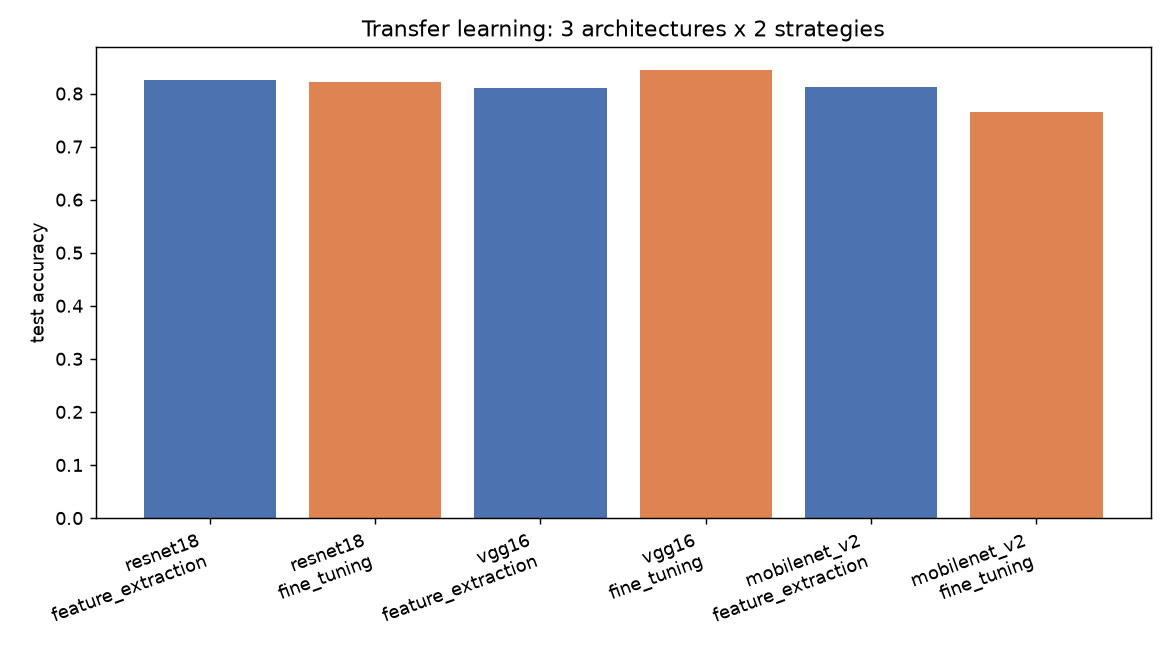
\includegraphics[width=0.95\textwidth]{figures/part_c_comparison.png}
    \caption{Test accuracy, all 6 architecture $\times$ strategy configurations.}
\end{figure}

\textbf{Best configuration: VGG16, fine-tuned (84.5\%).} Every one of the 6 configurations
beats the from-scratch custom CNN's 71.2\% (Part D quantifies the gap). Feature extraction
alone is already strong across all three architectures (81.0-82.5\%) -- ImageNet features
transfer well to CIFAR-10 objects even with zero backbone adaptation. Fine-tuning helps
substantially for VGG16 (+3.5 points) and marginally hurts for ResNet18 (-0.25) and
MobileNetV2 (-4.75) at these settings -- see C4 for why MobileNetV2 specifically regresses.

\textbf{C3 -- discriminative LR / gradual unfreezing.} ResNet18, all 4 stages unfrozen, 6
epochs, single shared backbone LR (1e-5) vs.\ per-stage discriminative LR (base 1e-4, decayed
by 0.3 per stage further from the head):

\begin{table}[H]
\centering
\begin{tabular}{lrrr}
\toprule
\textbf{Strategy} & \textbf{Test Acc} & \textbf{F1} & \textbf{Train time} \\
\midrule
Single LR (all layers) & 0.8425 & 0.8426 & 650s \\
Discriminative LR & \textbf{0.8550} & \textbf{0.8546} & \textbf{564s} \\
\bottomrule
\end{tabular}
\end{table}

Discriminative LR wins on \emph{both} accuracy (+1.25 points) and wall-clock time (86s
faster) -- smaller, more conservative updates to early (more-general, already-good) layers
apparently let the optimizer converge more directly than one shared LR fighting between
early-layer stability and late-layer adaptation needs.

\textbf{C4 -- preprocessing mismatch demo.} Identical frozen-feature-extraction pipeline on
ResNet18, run twice: once with correct ImageNet mean/std, once with deliberately wrong stats
(naive [0.5,0.5,0.5]/[0.5,0.5,0.5]), resolution and channel order held fixed and correct in
both:

\begin{table}[H]
\centering
\begin{tabular}{lr}
\toprule
\textbf{Normalization} & \textbf{Test Acc} \\
\midrule
Correct (ImageNet mean/std) & 0.8250 \\
Wrong (naive [0.5]$\times$3) & 0.7500 \\
\bottomrule
\end{tabular}
\caption{Accuracy drop from normalization mismatch alone: 7.5 points.}
\end{table}

Mismatched preprocessing degrades performance because the pretrained backbone's early-layer
filters were learned against a specific input distribution (ImageNet's per-channel
mean/std); feeding it inputs shifted/scaled differently pushes activations off the
distribution those filters were tuned for, degrading every downstream layer's features --
7.5 points is a substantial, measured cost for what looks like a small, easy-to-miss
implementation detail.

% ----------------------------------------------------------------
\section*{Part D: Comparative Analysis \& Ablation Study}

\textbf{D1 -- custom CNN vs.\ best transfer configuration.}

\begin{figure}[H]
    \centering
    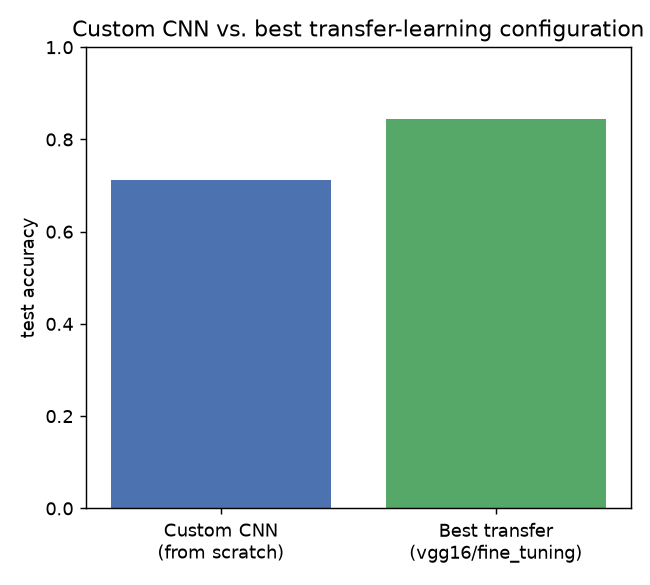
\includegraphics[width=0.55\textwidth]{figures/part_d_custom_vs_transfer.png}
    \caption{Custom CNN (from scratch) vs.\ best transfer-learning configuration (VGG16, fine-tuned).}
\end{figure}

\textbf{Absolute gap: 13.3 points (0.712 $\to$ 0.845); relative gap: 18.7\%.} This is the
clearest empirical evidence in this task of pretrained representations' value at small
dataset sizes: the custom CNN and best transfer model are evaluated on the same-size test
split, and the only substantive difference is that one starts from features learned on 1.2M
ImageNet images and the other starts from random initialization. 2{,}000-6{,}000 training
images is not enough to learn good low/mid-level visual features (edges, textures, simple
shapes) from scratch; transfer learning only has to adapt already-good features to
CIFAR-10's 10 classes.

\textbf{D2 -- unfreeze-depth ablation.} ResNet18, 0 (pure feature extraction) through 4
(fine-tune everything) unfrozen stages, 5 epochs each.

\begin{figure}[H]
    \centering
    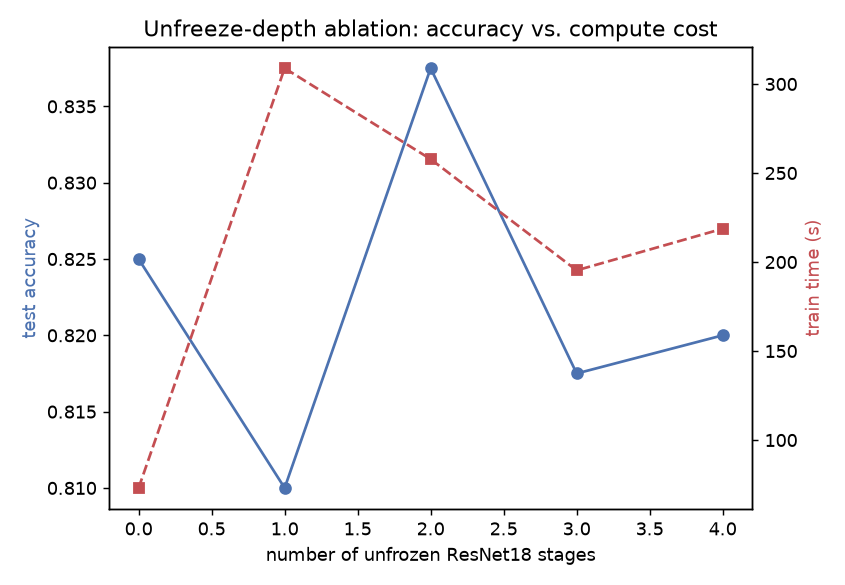
\includegraphics[width=0.75\textwidth]{figures/part_d_unfreeze_ablation.png}
    \caption{Unfreeze-depth ablation: test accuracy and training time vs.\ number of unfrozen stages.}
\end{figure}

\begin{table}[H]
\centering
\begin{tabular}{lrr}
\toprule
\textbf{Unfrozen stages} & \textbf{Test acc} & \textbf{Train time} \\
\midrule
0 (feature extraction) & 0.8250 & 73s \\
1 & 0.8100 & 309s \\
2 & \textbf{0.8375} & 258s \\
3 & 0.8175 & 195s \\
4 (fine-tune all) & 0.8200 & 219s \\
\bottomrule
\end{tabular}
\end{table}

The relationship is \textbf{non-monotonic}, not the naive "more unfrozen = better" story:
2 unfrozen stages is the best of the five, and 1 unfrozen stage is actually the
\emph{worst} -- worse than pure feature extraction (0 stages). A plausible explanation:
partially unfreezing without enough epochs to fully re-converge (5 epochs here, vs.\ C3's
6-epoch full-unfreeze run reaching much higher train accuracy) can leave a network in a
worse spot than either extreme -- too disturbed from its pretrained optimum to still coast
on frozen features, not trained long enough to reach a new one. This also cautions against
reading too much into any single ablation point without a convergence check.

\textbf{D3 -- architecture trade-offs.}

\begin{figure}[H]
    \centering
    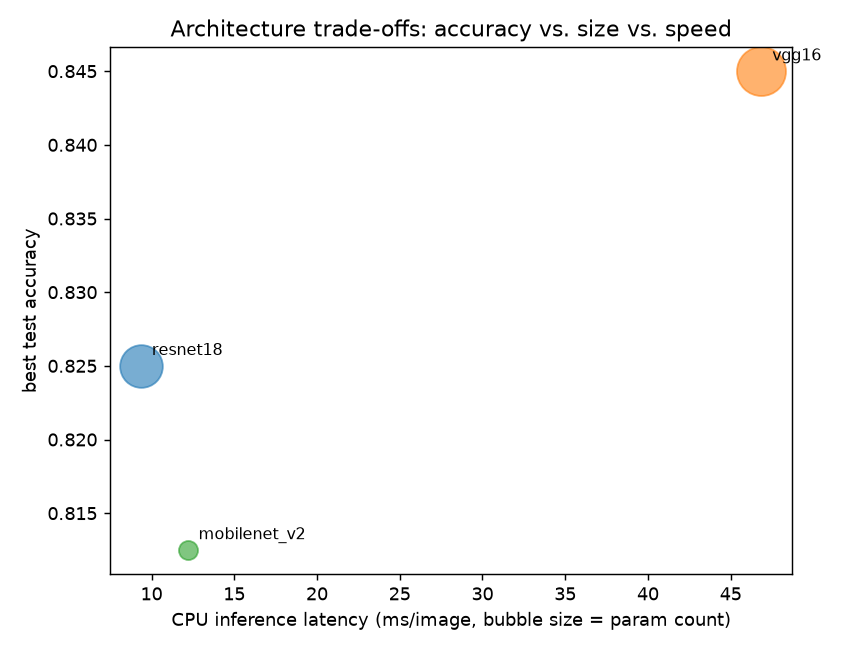
\includegraphics[width=0.7\textwidth]{figures/part_d_architecture_tradeoffs.png}
    \caption{Accuracy vs.\ CPU inference latency vs.\ backbone parameter count (bubble size).}
\end{figure}

\begin{table}[H]
\centering
\begin{tabular}{lrrr}
\toprule
\textbf{Architecture} & \textbf{Backbone params} & \textbf{Best test acc} & \textbf{CPU latency} \\
\midrule
ResNet18 & 11.18M & 0.8250 & 9.4ms/img \\
VGG16 & 14.72M & \textbf{0.8450} & 46.9ms/img \\
MobileNetV2 & \textbf{2.22M} & 0.8125 & \textbf{12.2ms/img} \\
\bottomrule
\end{tabular}
\end{table}

\textbf{Cloud service, no latency constraint}: \textbf{VGG16} -- highest accuracy (84.5\%),
and when nothing is waiting on a single request in real time, its 46.9ms/img latency and
14.7M-parameter size are irrelevant against batched cloud throughput. \textbf{On-device
mobile application}: \textbf{MobileNetV2} -- 6.6x fewer parameters than VGG16 (2.2M vs.\
14.7M, meaning a far smaller app footprint) and $\sim$4x lower latency (12.2ms vs.\ 46.9ms)
for only a 3.25-point accuracy cost versus VGG16; it is also, not coincidentally, the
architecture whose depthwise-separable convolutions were specifically designed for this
constraint. ResNet18 is the reasonable middle-ground default when neither extreme applies.

\textbf{D4 -- catastrophic forgetting and negative transfer.} No clear evidence of either.
If fine-tuning were catastrophically overwriting useful ImageNet features, deeper unfreezing
should degrade accuracy monotonically -- D2's ablation instead stays in an 81-84\% band with
no such trend. Negative transfer (pretrained features actively hurting vs.\ training from
scratch) also isn't observed: every one of Part C's 6 transfer configurations, including the
weakest (MobileNetV2 fine-tuning, 76.5\%), beats the from-scratch custom CNN's 71.2\%. The
one place something forgetting-\emph{adjacent} plausibly shows up is MobileNetV2's
fine-tuning underperforming its own feature-extraction result (76.5\% vs.\ 81.25\%, Part C2)
-- MobileNetV2's depthwise-separable blocks pack far fewer parameters per unfrozen stage than
ResNet18/VGG16's dense conv blocks, so the same backbone\_lr=1e-5 tuned to suit the other two
architectures may be relatively too aggressive for MobileNetV2's more parameter-efficient
layers, disturbing useful pretrained filters faster than a 2{,}000-image training set can
usefully re-fit them -- an architecture-specific LR-sensitivity effect, not textbook
catastrophic forgetting.

% ----------------------------------------------------------------
\section*{Part E: Documentation \& Reflection}

\textbf{E1.} Both final models saved as plain \texttt{state\_dict}s under \texttt{models/}:
the custom CNN as \texttt{custom\_cnn.pt} and the best transfer model as
\texttt{best\_transfer\_model.pt}. \texttt{part\_e\_reload\_demo.py} reloads both from disk
only (no in-memory state from training) and runs inference, confirming both work standalone.

\textbf{E2 -- pipeline summary.} Data: CIFAR-10, 10 classes, two subset sizes (6k/1k/1k for
the custom-CNN pipeline at 32$\times$32; 2k/400/400 for the transfer-learning pipeline at
128$\times$128, both class-balanced and cached to a shared index file so every part evaluates
on identical splits). Preprocessing: CIFAR-specific mean/std normalization for the custom
CNN, ImageNet mean/std for every pretrained backbone (Part C4 quantifies the cost of getting
this wrong). Training strategy: custom CNN uses AdamW (won a documented 6-config search) or
SGD+momentum with cosine-annealing or constant LR; transfer learning uses Adam throughout,
with frozen-backbone feature extraction training only a cached-feature linear head (cheap)
and fine-tuning unfreezing 1-4 backbone stages at a 100-1000x lower LR than the head.
Results: custom CNN 71.2\% test accuracy (392K params); best transfer configuration (VGG16,
fine-tuned) 84.5\% (13.3 points higher) at an 18x larger trained-parameter count and 34x
longer training time on CPU.

\textbf{E3 -- two non-trivial challenges.}

\emph{1. CIFAR-10's canonical download host was throttled to $\sim$200 bytes/sec.} Diagnosed
directly (a timed \texttt{curl}, not assumption) rather than just retrying: confirmed a
sustained throttle, not transient noise, then tested alternative hosts for the identical
data rather than switching blindly. The fast.ai S3 mirror served the same images at
$\sim$140KB/s (a $\sim$700x speedup). Resolved by writing an \texttt{ImageFolder}-based
loader in place of torchvision's pickle-format \texttt{CIFAR10} class, verified to produce
the identical 10 classes in the same alphabetical order before any training touched it.

\emph{2. Six-plus full CNN training runs on a CPU with no GPU is a fundamentally different
compute budget than one from-scratch model.} VGG16 fine-tuning alone took $\sim$28 minutes
for 6 epochs on a 2{,}000-image set. Diagnosed early via a small per-epoch timing check
before committing to the full 6-configuration $\times$ 2-ablation matrix, confirming
forward/backward compute -- not data loading -- was the actual bottleneck (consistent with
CPU matrix-multiply throughput, not I/O, being the limiting factor). Resolved by
aggressively subsetting at every stage that touches a full pretrained backbone (2k/400/400
images, 128$\times$128 resolution) and caching frozen-backbone features once per
feature-extraction run instead of recomputing them every epoch, turning a many-hour job into
one completing within a single working session.

\textbf{E4 -- reflection.} Transfer learning is preferable whenever labeled data is scarce
relative to problem difficulty -- exactly this task's regime, and the 13.3-point Part D gap
is direct empirical evidence of that value at this dataset size: 2{,}000 images is not
enough to learn good low/mid-level visual features from random initialization, but ImageNet
pretraining already supplies them, leaving only class-specific adaptation to learn. Training
a custom architecture from scratch remains the better choice when (a) the target domain is
far enough from natural images that ImageNet features transfer poorly (medical scans,
satellite imagery, spectrograms), (b) inference-time constraints demand an architecture
shape no pretrained model zoo offers, or (c) enough labeled data and compute exist that a
from-scratch model's capacity can be fully exploited without a pretrained initialization's
inductive bias becoming a ceiling rather than a boost -- none of which held in this task's
compute-constrained, small-subset setting.

\end{document}
